% Options for packages loaded elsewhere
\PassOptionsToPackage{unicode}{hyperref}
\PassOptionsToPackage{hyphens}{url}
\PassOptionsToPackage{dvipsnames,svgnames,x11names}{xcolor}
%
\documentclass[
  letterpaper,
  DIV=11,
  numbers=noendperiod]{scrartcl}

\usepackage{amsmath,amssymb}
\usepackage{iftex}
\ifPDFTeX
  \usepackage[T1]{fontenc}
  \usepackage[utf8]{inputenc}
  \usepackage{textcomp} % provide euro and other symbols
\else % if luatex or xetex
  \usepackage{unicode-math}
  \defaultfontfeatures{Scale=MatchLowercase}
  \defaultfontfeatures[\rmfamily]{Ligatures=TeX,Scale=1}
\fi
\usepackage{lmodern}
\ifPDFTeX\else  
    % xetex/luatex font selection
\fi
% Use upquote if available, for straight quotes in verbatim environments
\IfFileExists{upquote.sty}{\usepackage{upquote}}{}
\IfFileExists{microtype.sty}{% use microtype if available
  \usepackage[]{microtype}
  \UseMicrotypeSet[protrusion]{basicmath} % disable protrusion for tt fonts
}{}
\makeatletter
\@ifundefined{KOMAClassName}{% if non-KOMA class
  \IfFileExists{parskip.sty}{%
    \usepackage{parskip}
  }{% else
    \setlength{\parindent}{0pt}
    \setlength{\parskip}{6pt plus 2pt minus 1pt}}
}{% if KOMA class
  \KOMAoptions{parskip=half}}
\makeatother
\usepackage{xcolor}
\setlength{\emergencystretch}{3em} % prevent overfull lines
\setcounter{secnumdepth}{5}
% Make \paragraph and \subparagraph free-standing
\ifx\paragraph\undefined\else
  \let\oldparagraph\paragraph
  \renewcommand{\paragraph}[1]{\oldparagraph{#1}\mbox{}}
\fi
\ifx\subparagraph\undefined\else
  \let\oldsubparagraph\subparagraph
  \renewcommand{\subparagraph}[1]{\oldsubparagraph{#1}\mbox{}}
\fi


\providecommand{\tightlist}{%
  \setlength{\itemsep}{0pt}\setlength{\parskip}{0pt}}\usepackage{longtable,booktabs,array}
\usepackage{calc} % for calculating minipage widths
% Correct order of tables after \paragraph or \subparagraph
\usepackage{etoolbox}
\makeatletter
\patchcmd\longtable{\par}{\if@noskipsec\mbox{}\fi\par}{}{}
\makeatother
% Allow footnotes in longtable head/foot
\IfFileExists{footnotehyper.sty}{\usepackage{footnotehyper}}{\usepackage{footnote}}
\makesavenoteenv{longtable}
\usepackage{graphicx}
\makeatletter
\def\maxwidth{\ifdim\Gin@nat@width>\linewidth\linewidth\else\Gin@nat@width\fi}
\def\maxheight{\ifdim\Gin@nat@height>\textheight\textheight\else\Gin@nat@height\fi}
\makeatother
% Scale images if necessary, so that they will not overflow the page
% margins by default, and it is still possible to overwrite the defaults
% using explicit options in \includegraphics[width, height, ...]{}
\setkeys{Gin}{width=\maxwidth,height=\maxheight,keepaspectratio}
% Set default figure placement to htbp
\makeatletter
\def\fps@figure{htbp}
\makeatother
% definitions for citeproc citations
\NewDocumentCommand\citeproctext{}{}
\NewDocumentCommand\citeproc{mm}{%
  \begingroup\def\citeproctext{#2}\cite{#1}\endgroup}
\makeatletter
 % allow citations to break across lines
 \let\@cite@ofmt\@firstofone
 % avoid brackets around text for \cite:
 \def\@biblabel#1{}
 \def\@cite#1#2{{#1\if@tempswa , #2\fi}}
\makeatother
\newlength{\cslhangindent}
\setlength{\cslhangindent}{1.5em}
\newlength{\csllabelwidth}
\setlength{\csllabelwidth}{3em}
\newenvironment{CSLReferences}[2] % #1 hanging-indent, #2 entry-spacing
 {\begin{list}{}{%
  \setlength{\itemindent}{0pt}
  \setlength{\leftmargin}{0pt}
  \setlength{\parsep}{0pt}
  % turn on hanging indent if param 1 is 1
  \ifodd #1
   \setlength{\leftmargin}{\cslhangindent}
   \setlength{\itemindent}{-1\cslhangindent}
  \fi
  % set entry spacing
  \setlength{\itemsep}{#2\baselineskip}}}
 {\end{list}}
\usepackage{calc}
\newcommand{\CSLBlock}[1]{\hfill\break\parbox[t]{\linewidth}{\strut\ignorespaces#1\strut}}
\newcommand{\CSLLeftMargin}[1]{\parbox[t]{\csllabelwidth}{\strut#1\strut}}
\newcommand{\CSLRightInline}[1]{\parbox[t]{\linewidth - \csllabelwidth}{\strut#1\strut}}
\newcommand{\CSLIndent}[1]{\hspace{\cslhangindent}#1}

\KOMAoption{captions}{tableheading}
\makeatletter
\@ifpackageloaded{caption}{}{\usepackage{caption}}
\AtBeginDocument{%
\ifdefined\contentsname
  \renewcommand*\contentsname{Table of contents}
\else
  \newcommand\contentsname{Table of contents}
\fi
\ifdefined\listfigurename
  \renewcommand*\listfigurename{List of Figures}
\else
  \newcommand\listfigurename{List of Figures}
\fi
\ifdefined\listtablename
  \renewcommand*\listtablename{List of Tables}
\else
  \newcommand\listtablename{List of Tables}
\fi
\ifdefined\figurename
  \renewcommand*\figurename{Figure}
\else
  \newcommand\figurename{Figure}
\fi
\ifdefined\tablename
  \renewcommand*\tablename{Table}
\else
  \newcommand\tablename{Table}
\fi
}
\@ifpackageloaded{float}{}{\usepackage{float}}
\floatstyle{ruled}
\@ifundefined{c@chapter}{\newfloat{codelisting}{h}{lop}}{\newfloat{codelisting}{h}{lop}[chapter]}
\floatname{codelisting}{Listing}
\newcommand*\listoflistings{\listof{codelisting}{List of Listings}}
\makeatother
\makeatletter
\makeatother
\makeatletter
\@ifpackageloaded{caption}{}{\usepackage{caption}}
\@ifpackageloaded{subcaption}{}{\usepackage{subcaption}}
\makeatother
\ifLuaTeX
  \usepackage{selnolig}  % disable illegal ligatures
\fi
\usepackage{bookmark}

\IfFileExists{xurl.sty}{\usepackage{xurl}}{} % add URL line breaks if available
\urlstyle{same} % disable monospaced font for URLs
\hypersetup{
  pdftitle={Iliocostalis},
  pdfauthor={Nathaniel Giovanni Yomogida, SPT; Chloë Anne Kerstein, SPT},
  colorlinks=true,
  linkcolor={blue},
  filecolor={Maroon},
  citecolor={Blue},
  urlcolor={Blue},
  pdfcreator={LaTeX via pandoc}}

\title{Iliocostalis}
\author{Nathaniel Yomogida, SPT \and Chloë Kerstein, SPT}
\date{}

\begin{document}
\maketitle

\renewcommand*\contentsname{Table of contents}
{
\hypersetup{linkcolor=}
\setcounter{tocdepth}{3}
\tableofcontents
}
\section{OIAN}\label{oian}

\begin{figure}

\centering{

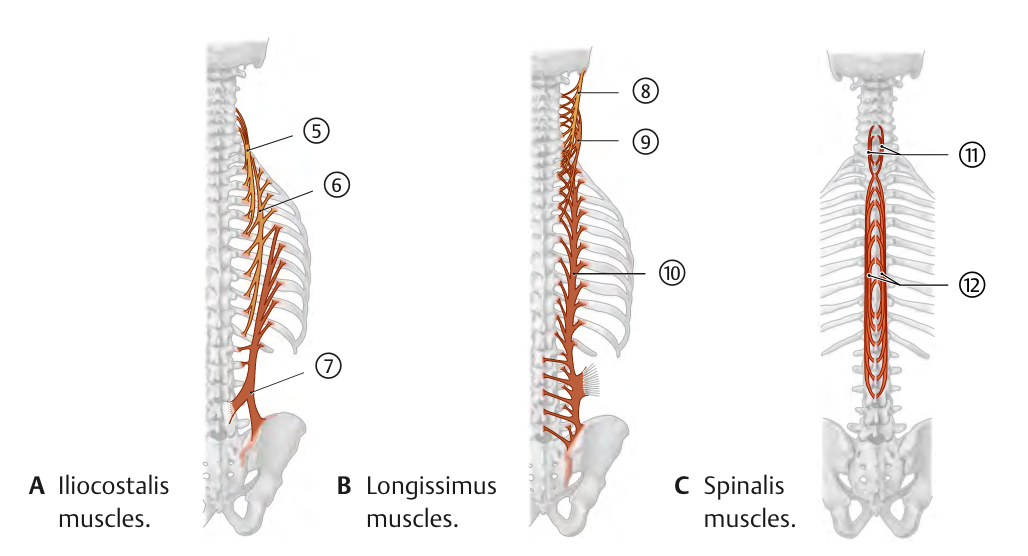
\includegraphics{../../../../Alchemy Archive/Anatomy/OIANs/images/3.9a schematic intermediate back muscles gilroyAtlasAnatomy2020.png}

}

\caption{\label{fig-schematicintermediatebackmm39gilroyAtlasAnatomy2020}Schematic
view of the intermediate intrinsic muscles of the back (Erector
spinae)\textsuperscript{\citeproc{ref-gilroyAtlasAnatomy2020}{1}}}

\end{figure}%

\begin{figure}

\centering{

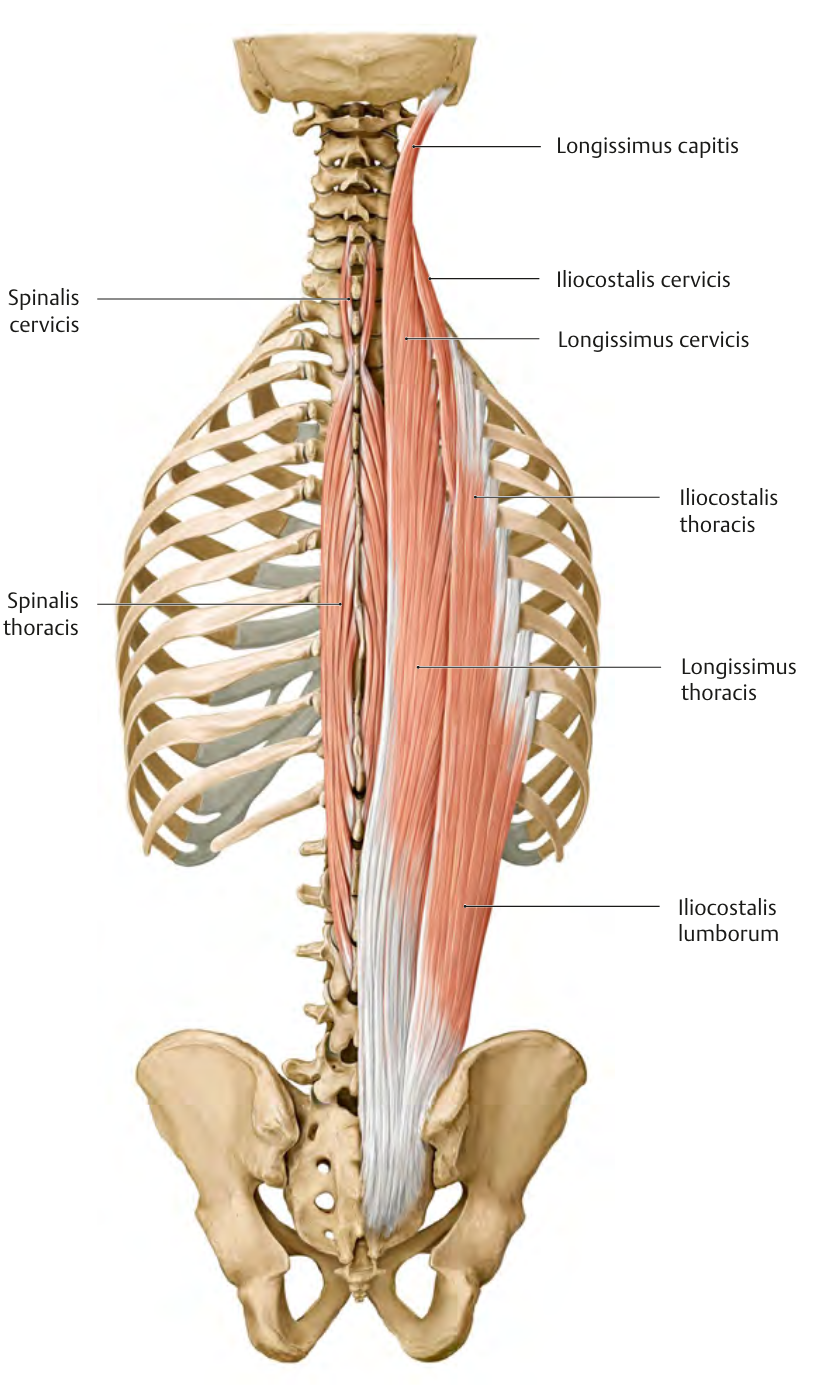
\includegraphics{../../../../Alchemy Archive/Anatomy/OIANs/images/310b intermediate back muscles gilroyAtlasAnatomy2020.png}

}

\caption{\label{fig-intermediatebackmm310gilroyAtlasAnatomy2020}Intermediate
intrinsic muscles of the back / Erector spinae (Posterior
view)\textsuperscript{\citeproc{ref-gilroyAtlasAnatomy2020}{1}}}

\end{figure}%

\begin{longtable}[]{@{}
  >{\raggedright\arraybackslash}p{(\columnwidth - 8\tabcolsep) * \real{0.1538}}
  >{\raggedright\arraybackslash}p{(\columnwidth - 8\tabcolsep) * \real{0.2051}}
  >{\raggedright\arraybackslash}p{(\columnwidth - 8\tabcolsep) * \real{0.1795}}
  >{\raggedright\arraybackslash}p{(\columnwidth - 8\tabcolsep) * \real{0.2564}}
  >{\raggedright\arraybackslash}p{(\columnwidth - 8\tabcolsep) * \real{0.2051}}@{}}
\caption{Iliocostalis OIAN}\tabularnewline
\toprule\noalign{}
\begin{minipage}[b]{\linewidth}\raggedright
Muscle
\end{minipage} & \begin{minipage}[b]{\linewidth}\raggedright
Origin
\end{minipage} & \begin{minipage}[b]{\linewidth}\raggedright
Insertion
\end{minipage} & \begin{minipage}[b]{\linewidth}\raggedright
Nerve
\end{minipage} & \begin{minipage}[b]{\linewidth}\raggedright
Action
\end{minipage} \\
\midrule\noalign{}
\endfirsthead
\toprule\noalign{}
\begin{minipage}[b]{\linewidth}\raggedright
Muscle
\end{minipage} & \begin{minipage}[b]{\linewidth}\raggedright
Origin
\end{minipage} & \begin{minipage}[b]{\linewidth}\raggedright
Insertion
\end{minipage} & \begin{minipage}[b]{\linewidth}\raggedright
Nerve
\end{minipage} & \begin{minipage}[b]{\linewidth}\raggedright
Action
\end{minipage} \\
\midrule\noalign{}
\endhead
\bottomrule\noalign{}
\endlastfoot
\href{../../../../Alchemy\%20Archive/Anatomy/OIANs/Muscles\%20of\%20the\%20back/iliocostalis.qmd}{Iliocostalis
cervicis} & 3rd-7th ribs & C4-C6 TP &
\href{\%7B\%7B\%3C\%20var\%20ref-spinal-nerves.path\%20\%3E\%7D\%7D}{Spinal
nn.~} C8-L1 (Post rami, lateral branches) & \textbf{BIL:} Extends spine;
\textbf{UNIL:} I/L spine lat-flexion \\
\href{../../../../Alchemy\%20Archive/Anatomy/OIANs/Muscles\%20of\%20the\%20back/iliocostalis.qmd}{Iliocostalis
thoracis} & 7-12th ribs & 1st-6th ribs &
\href{\%7B\%7B\%3C\%20var\%20ref-spinal-nerves.path\%20\%3E\%7D\%7D}{Spinal
nn.} C8-L1 (Post rami, lateral branches) & \textbf{BIL:} Extends spine;
\textbf{UNIL:} I/L spine lat-flexion \\
\href{../../../../Alchemy\%20Archive/Anatomy/OIANs/Muscles\%20of\%20the\%20back/iliocostalis.qmd}{Iliocostalis
lumborum} & Sacrum, iliac crest, lumbar vertebrae SP; lower thoracic
vertebrae TP & 6-12th ribs, thoracolumbar fascia (posterior layer),
upper lumbar vertebrae (TP) &
\href{\%7B\%7B\%3C\%20var\%20ref-spinal-nerves.path\%20\%3E\%7D\%7D}{Spinal
nn.~} C8-L1 (Post rami, lateral branches) & \textbf{BIL:} Extends spine;
\textbf{UNIL:} I/L spine lat-flexion \\
\end{longtable}

\section{Iliocostalis Cervicis}\label{iliocostalis-cervicis}

\subsection{Origin}\label{origin}

3rd-7th ribs\textsuperscript{\citeproc{ref-gilroyAtlasAnatomy2020}{1}}

\subsection{Insertion}\label{insertion}

C4-C6 TP\textsuperscript{\citeproc{ref-gilroyAtlasAnatomy2020}{1}}

\subsection{Innervation}\label{innervation}

\href{../../../../Alchemy\%20Archive/Anatomy/Nerves/spinal_nerves.qmd}{Spinal
nn.} C8-L1 (Post rami, lateral
branches)\textsuperscript{\citeproc{ref-gilroyAtlasAnatomy2020}{1}}

\subsection{Action}\label{action}

\section{Iliocostalis Thoracis}\label{iliocostalis-thoracis}

\subsection{Origin}\label{origin-1}

7-12th ribs\textsuperscript{\citeproc{ref-gilroyAtlasAnatomy2020}{1}}

\subsection{Insertion}\label{insertion-1}

1st-6th ribs\textsuperscript{\citeproc{ref-gilroyAtlasAnatomy2020}{1}}

\subsection{Innervation}\label{innervation-1}

\href{../../../../Alchemy\%20Archive/Anatomy/Nerves/spinal_nerves.qmd}{Spinal
nn.} C8-L1 (Post rami, lateral
branches)\textsuperscript{\citeproc{ref-gilroyAtlasAnatomy2020}{1}}

\subsection{Action}\label{action-1}

\section{Iliocostalis Lumborum}\label{iliocostalis-lumborum}

\subsection{Origin}\label{origin-2}

Sacrum, iliac crest, lumbar vertebrae SP; lower thoracic vertebrae
TP\textsuperscript{\citeproc{ref-gilroyAtlasAnatomy2020}{1}}

\subsection{Insertion}\label{insertion-2}

6-12th ribs, thoracolumbar fascia (posterior layer), upper lumbar
vertebrae (TP)\textsuperscript{\citeproc{ref-gilroyAtlasAnatomy2020}{1}}

\subsection{Innervation}\label{innervation-2}

\href{../../../../Alchemy\%20Archive/Anatomy/Nerves/spinal_nerves.qmd}{Spinal
nn.} C8-L1 (Post rami, lateral
branches)\textsuperscript{\citeproc{ref-gilroyAtlasAnatomy2020}{1}}

\subsection{Action}\label{action-2}

\begin{itemize}
\tightlist
\item
  \textbf{Bilateral:} Extends
  spine\textsuperscript{\citeproc{ref-gilroyAtlasAnatomy2020}{1}}
\item
  \textbf{Unilateral:} I/L spine
  lat-flexion\textsuperscript{\citeproc{ref-gilroyAtlasAnatomy2020}{1}}
\end{itemize}

\section{Muscle groups}\label{muscle-groups}

Iliocostalis is part of the \href{}{Intermediate intrinsic back muscles
(erector spinae)}

\section{Palpation}\label{palpation}

\section*{Clinical significance}\label{clinical-significance}
\addcontentsline{toc}{section}{Clinical significance}

\phantomsection\label{refs}
\begin{CSLReferences}{0}{1}
\bibitem[\citeproctext]{ref-gilroyAtlasAnatomy2020}
\CSLLeftMargin{1. }%
\CSLRightInline{Gilroy AM, MacPherson BR, Wikenheiser JC, Voll MM,
Wesker K, Schünke M, eds. \emph{Atlas of Anatomy}. 4th ed. {Thieme};
2020.}

\end{CSLReferences}



\end{document}
